\chapter{The Standard Analysis Method for Resonance Finding}
\label{StandardAnalysisMethod}

\epigraph{\textit{But the truth can be re-found; most often it has already been written elsewhere.}}{--Jacques Lacan, Ecrits}

%TODO Adding Monte Carlo methods \\Edited
%TODO Gaussian process motivation
%TODO Fit function + swift method
%TODO Bayesian method for limit setting
%TODO Add fig:bump


\section{Introduction}
All three analyses presented in this thesis fall into the resonance search category, which are analyses that look for bumps like excesses on top of smooth backgrounds. The method is simple in its experimental signature~\ref{fig:bump} and theoretical calculation. Many particles have been discovered that way before, which include the W~\cite{Arnison:142059}, Z, and the Higgs boson. It is therefore believed that the method has great potential in making new future discoveries. This chapter describes the analysis methods used in performing the analyses covered in chapter~\ref{chapter:dijet} and ~\ref{chapter:dimuon}. 


These analyses perform searches in the resonance mass variable, which numerically is the addition of the 4-vector of the two candidate final state particles, and reconstruct a resonance candidate. 

\begin{figure}[!htb]
    \begin{center}
        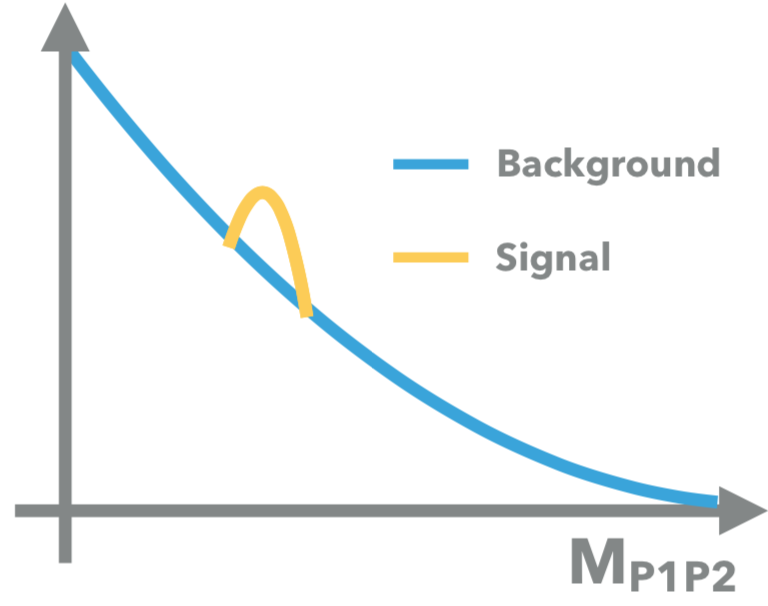
\includegraphics[width=0.3\textwidth]{figures/chapter_analysismethod/resonance}
        \caption{
            This cartoon illustrates a typical resonance finding experimental signature in the resonance mass variable. 
        }
        \label{fig:bump}
    \end{center}
\end{figure}
\FloatBarrier

The chapter below provides a recipe for a resonance finding analysis: first, data is properly prepared before the statistical analysis, a summary on the basic event selection, trigger chain building, and signal sensitivity cut test are discussed in Section~\ref{sec:dataprep}. Second, in both the dimuon~\ref{chapter:dimuon} and dijetISR~\ref{chapter:dijet} channels, the background event size is large compared to what can be reliably generated by Monte Carlo, therefore the "smoothness"
feature in the resonance mass projection is relied upon to estimate the background by data-driven methods, the details of the different smooth background estimation method and their verifications are given in Section~\ref{sec:backgroundest}. Lastly, the search for resonances as excesses is quantified statistically. Two separate tests, one on excess finding, and the other one on signal strenght upper limit setting are found The details on the analysis procedure and the derivation
and justification of the methods are discussed in Section~\ref{section:stats}. 

\section{Simulated Physics Events(Monte Carlo)}
In this analysis, simulated physics events(Monte Carlo) are used to study the optimal signal sensitivity cuts for event selection, verifying the validity of the data-driven background estimation strategies as well as the different systematics.
The default ATLAS event generator is PYTHIA, it is used to simulate the proton-proton collision, the tree level outcome, the hadronization, the fragmentation as well as the showering~\cite{PYTHIA}. It uses different \textit{tunes}, which are models and their parameters to estimate effect of pile-up and effect of simulated ``next-to-leading-order" showering. Other than PYTHIA, the PowHeg generator~\cite{oleari2010powheg} and the NLOJet++~\cite{nagynlojet++} are also used. They could provide more accurate results for certain physics processes. In the analyses listed in this thesis, events generated by different generators are only used for cross checks and systematics. 
The detector effect is simulated by GEANT4~\cite{Agostinelli:602040}. The shower particle's interaction with detector material is simulated to produce detector effect like those of the physics events.



\section{Data Preparation}
\label{sec:dataprep}
The data of the analyses discussed in this chapter came from LHC proton-proton collision data, collected from the ATLAS detector and its triggering hardware and software discussed in chapter~\cite{chapter:ATLAS}. The data collected as energy deposit and tracks are analyzed and collected analysis objects as discussed in~\cite{chapter:common_analysis_objects}. After that, the dataset goes through several more steps in data preparation before getting analyzed for resonance finding in the chapter: the following is a short outline of how data are being prepared for the analyses.

First trigger chains that contain target events are studied to maximize the size of the dataset being studied; after that, the data is processed with the optimal analysis object working points applied, then, event cuts are introduce to maximize the signal sensitivity while cutting down on the background; in addition, binning on the target spectrum(in the case of analyses in this thesis, the resonance mass spectrum) is found for optimal detector resolution and signal sensitivity, as discussed in
Section~\ref{sec:binning}. A final check on that compares the data and MC is performed on control regions perpendicular to the signal region be done before the statistical analysis. An agreement up to a certain margin ensures both the previous steps in data preparation are likely done correctly and that the MC is close enough to data and can be used for different preparatory studies for the background estimation and binning strategies. After all the data preparation steps are done, a target signal spectrum is available to be analyzed statistically for resonances. 

\subsection{Binning Strategy} 
\label{sec:binning}

To prepare a mass spectrum, the data must be properly binned. The bins have to be narrower than the width of the expected signal, as this would minimize the possibility of mistaking fluctuation as an excess and improve characterization of the signal.

The binning is done through the mass spectrum resolution finding of the target spectrum. The mass resolution is found through a width-to-mean($\frac{\mu}{sigma}$) Gaussian fit on the $m^{reco}/m^{truth}$ on the four-vector addition of the two candidate final state particles. The truth particles came from Pythia generation whereas the reconstructed value came from the GEANT4 detector reconstruction. A Gaussian fit is performed to find the mean ($\mu$) and the width($\sigma$).

A uniform binning is chosen for the dimuon analysis, as it would make the background estimation more simplified. For the dijet analysis, to cope with the low statistics in the high mass region, variable bin size based on detector resolution is used. 

\section{Background Modeling}
\label{sec:backgroundest}
After the dataset has been prepared, the spectrum is ready to be analyzed to search for resonances. In order to analyze statistically whether there is an excess of event beyond the Standard Model prediction, a reliable prediction of the Standard Model events in the signal region along with its statistical error is needed. From an accurate estimation of the background, statistical tests can then make statement on whether an excess of events, a telling signature of a resonance, are seen in data.
The step to estimate background Standard Model events is known as background estimation.
    Many considerations goes into background modeling for an analysis. Accuracy, availability, size of the estimation error and ease of implementation are all factors to be considered. In ATLAS these following methods are recommended for background modeling in order of descending preference:
    First, the background estimation can be found through the MC generation of the events when the simulation is reliable and inexpensive for data generation. Second, in cases where the MC generated is low in event count but reliable in shape, an alternative estimation could be done through scaling up the template from MC. As the case of these resonance search analyses presented in this thesis, neither are there enough MC events nor are the shape of the MC event physically reliable, another class of methods of background estimation needs to be explored, all relying on the ``smoothness" feature of the background events. These include the fit function method, the expanded sliding window fit method(SWiFT) and the Gaussian Process method.
    Traditionally, the fit function method and SWiFT are both used for background estimation in the dijet and dilepton final state searches. They both rely on fit functions produced from collider data from older experiments. They do not perform well when collision energy elevates or when luminosity increases exponentially revealing more features not previously captured. The steps to validating the background estimation method is also tedious and difficult.
    In view of these limitations, a method based on Gaussian Process, which explores the use of a class of function is developed~\cite{frate2017modeling}. It provides more flexibility than the traditional method and can be applied to a wide class of resonance finding searches with minimal reliance on fit functions. 
    In the following section, the fit function method, the SWiFT method(used for the dijet-resolved analysis), and the Gaussian Process method(used for the dimuon analysis) are discussed in detail. 

\subsection{Fit Functions/Global Fit}
\label{sec:fitfunction}
    The fit function method utilizes a class of fit functions are found to used to describe the distribution of the dijet/dilepton mass spectrum background. The most commonly used forms are cited as the following~\cite{ATL-PHYS-PUB-2020-028}. The selected fit functions are all resistant to capturing of localized excess and features that a narrow resonance would look like. They are generally known as ``smooth".

    \begin{itemize}

    \item \textbf{Polynomial}
        \begin{equation}
            f(m)= a_0 + a_{1}m + a_{2}m^{2}+...
        \end{equation} Here, m is the resonance mass, and $a_{i}$ are the different parameters.
    \item \textbf{Power Laws}
        \begin{equation}
            f(m)= a_{0}m^{b}
        \end{equation}

    \item \textbf{Exponentials}
        \begin{equation}
            f(m) = a_{0}(exp^{-b_{0}m} +a_{1}e^{-b_{1}m}+...
        \end{equation}

    \end{itemize}

From the above foundation, a list of historic fit functions has been developed over the years for the dijet/dilepton search~\cite{Pachal:2063032}.
    %TODO cite 

    \begin{equation}
        \frac{p_{0}}{m^{p_{1}}}exp-(p_{2}m+p_{3}m^{2})
    \end{equation}~\cite{UA2:1990gao}

    \begin{equation}
        \frac{p_{0}}{m^{p_{1}}}(1-\frac{m}{\sqrt{s}})p_{2}
    \end{equation}~\cite{1995}

    \begin{equation}
        \frac{p_{0}}{m^{p_{1}}}(1-\frac{m}{\sqrt{s}}+)p_{2}
    \end{equation}~\cite{b582dc2d9c234174bfe2adbc9729bf42}

    \begin{equation}
        p_{0}(1-x)^p_{1}x^{p_{2}+p_{3}ln(x)}
        \end{equation}, where x is $\frac{x}{\sqrt{s}}$ ~\cite{2009}

    \begin{equation}
        (1-x)^{p_{0}}x^{p1+p2ln(x)}
    \end{equation},where x is $\frac{x}{\sqrt{s}}$~\cite{2014}

\subsubsection{Cross-validation}
    A k-fold cross validation is often used to ensure the fit function is chosen correctly. In the procedure, the original dataset is divided into k different equal event size subsets through a random draw from the original dataset. Each of these subsets are tested by the candidate fit function. From the fit test statistics and pseudo-experiment and fit done, a background fit p-value is found for each of the k subset of data. The p-values can be averaged for a statement on the background fit and the best background fit function can be chosen that way. 

    While the fit function is relatively easy to implement. It's highly restrictive for complicated background shapes since it's low in flexibility, the function is also ad hoc and generally doesn't include much information about the physics of the underlying spectrum~\cite{ATL-PHYS-PUB-2020-028}. When the increase luminosity of the LHC dataset lead to difficulties in fitting the background accurately, SWiFT and Gaussian Process are developed for the challenge. 

    \subsection{Sliding window fit(SWiFT)}
    When the simple fit function failed to model the data, SWiFT can increase the fit flexibility and the degree of freedom by fitting windows along the spectrum. The SWiFT window fitting procedure is summarized as below:
    1. A global fit is performed in the overall spectrum. Only when the overall $\chi^{2}$ p-value goes below the fit threshold, SWiFT is attempted. Otherwise, the procedure ends in this step and a global fit method will be used. 
    2. The SWiFT fit will start with the maximum sized window, which is the size of the bins of the entire spectrum minus one. The window scan start from the lowest mass region along the spectrum. A fit is performed in the window. This estimates the spectrum up to the middle point the window.
    3. The window moves up by one bin along the resonance mass spectrum(to the right). Another fit is reperformed. The prediction up to the middle of the window(in one bin) is added to the prediction in step 2. 
    4. Step 3 is repeated, until the end of the spectrum is reached. The final fit is checked against the threshold p value of the $\chi^{2}$. If the fit $\chi^{2}$ is above the designated threshold, the background estimation ends. Otherwise, the window size is further reduced by one bin, and step 2 and 3 is repeated until either a fit above the test statistics threshold is found or the minimum window size is reached. The minimum window size is defined by the signal injection test discussed below~\ref{sec:signalInjection}.

    Figure~\ref{fig:swift} here shows a doodle on the sliding window method and detailed unblinding procedure. 
    While the SWiFT can provide extra flexibility to the fit, it is also prone to becoming too flexible where the signal could be fitted away along with the background. A carefully designed unblinding procedure is used. Figure~\ref{fig:unblinding} shows a sample unblinding procedure used in the dijetISR resolved analysis. 

\begin{figure}[!htb]
    \begin{center}
        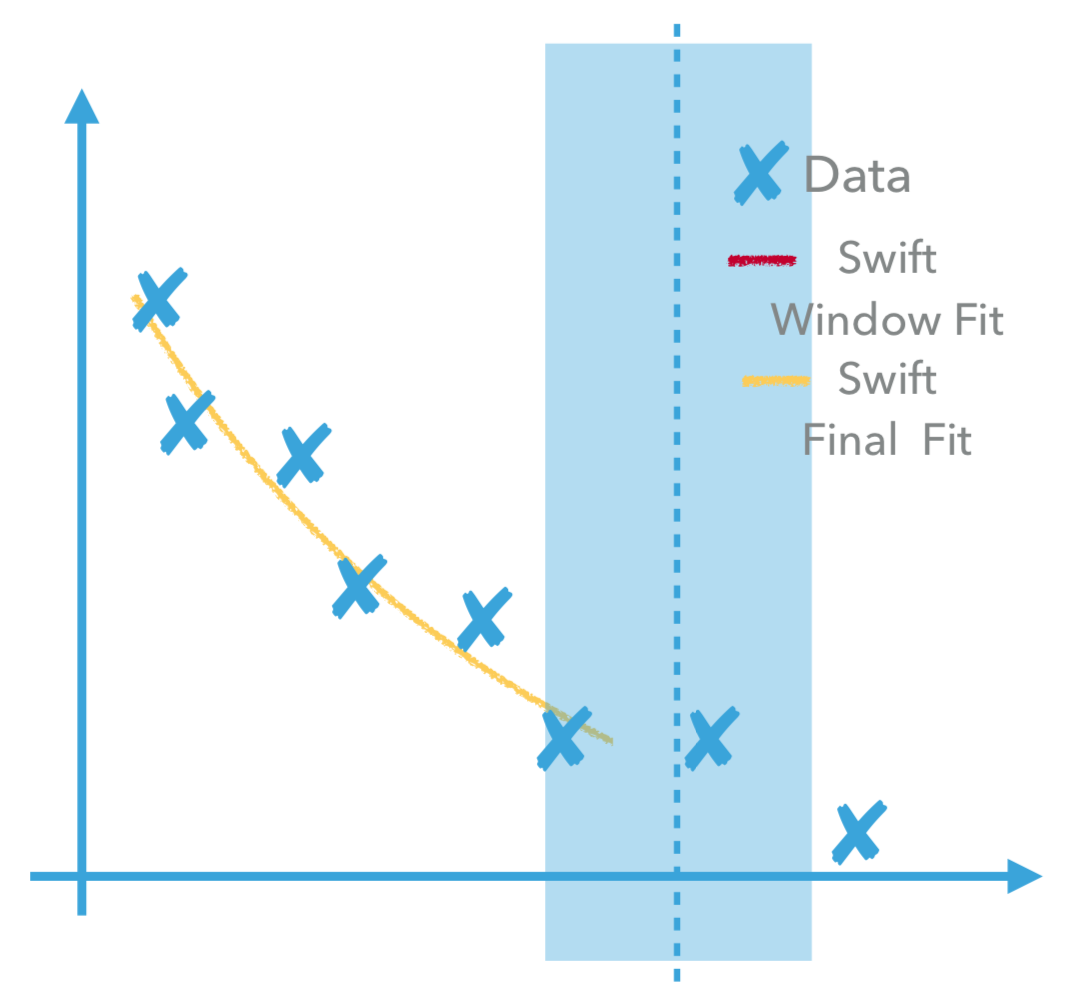
\includegraphics[width=0.3\textwidth]{figures/chapter_analysismethod/swift2}
        \caption{
            This figure shows a doodle on the procedure of the sliding window fit. 
        }
        \label{fig:swift}
    \end{center}
\end{figure}
\FloatBarrier

\begin{figure}[!htb] \begin{center}
        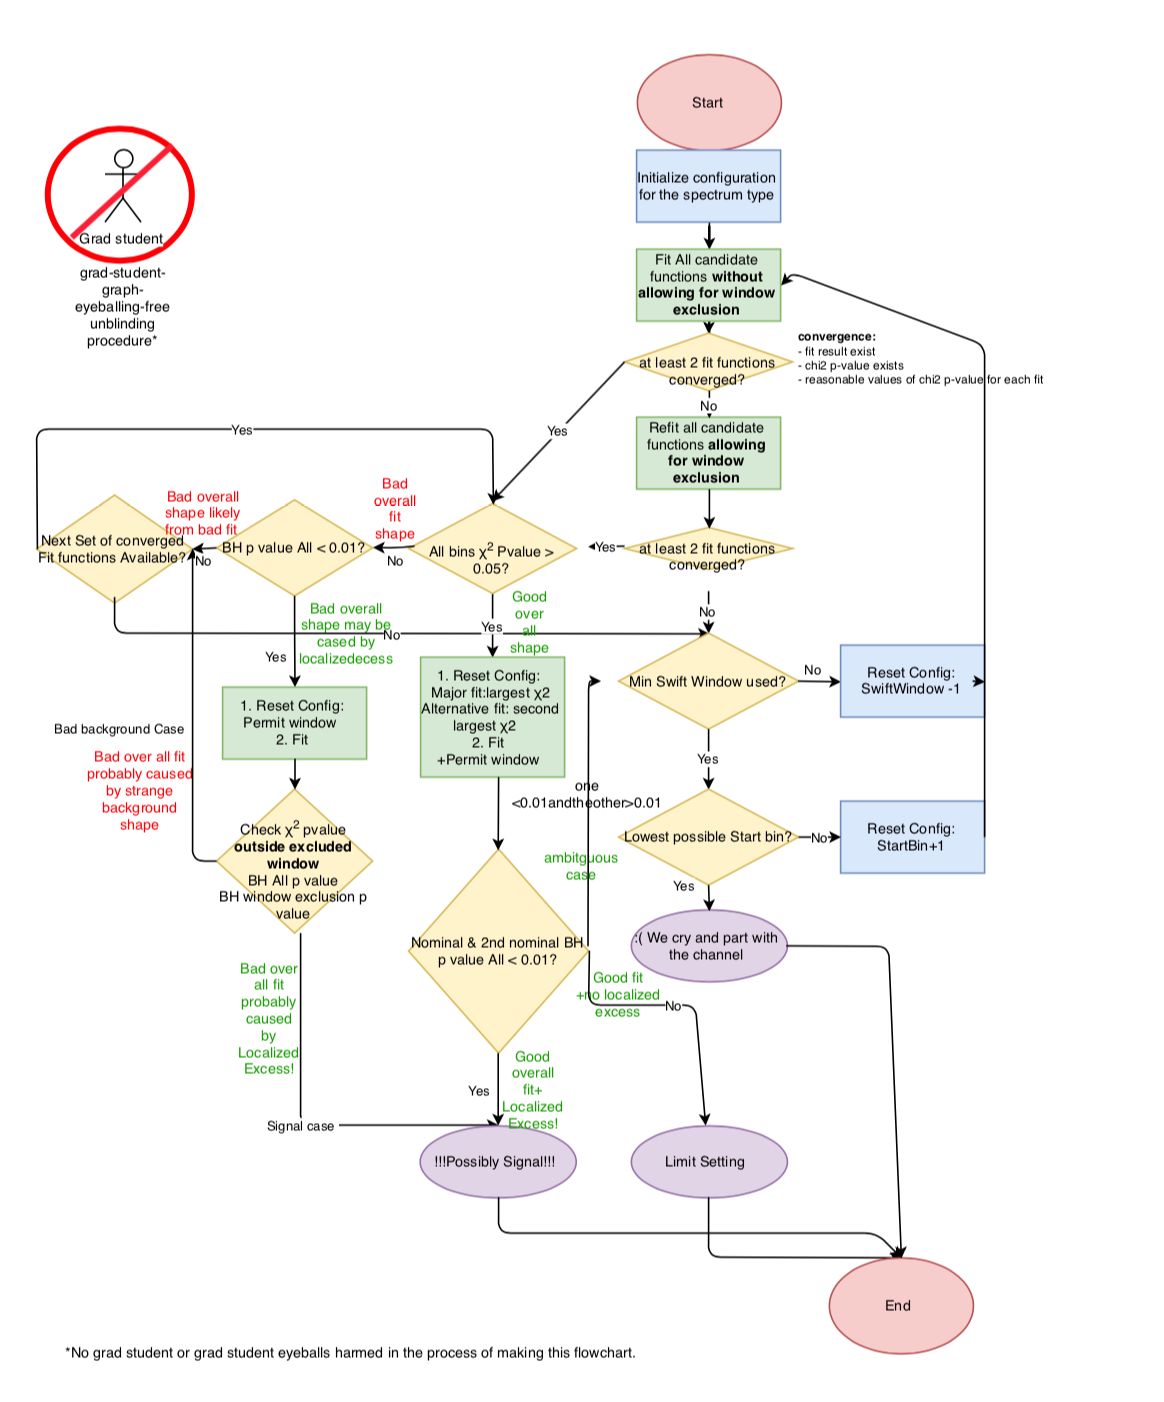
\includegraphics[width=1.05\textwidth]{figures/chapter_analysismethod/swift_unblindingflowchart}
        \caption{
            This figure shows a doodle on the procedure on the unblinding using SWiFT.
        }
        \label{fig:unblinding}
    \end{center}
\end{figure}
\FloatBarrier
    
    \subsection{Gaussian Process} 

    Gaussian process background prediction is done through Bayesian inference. Unlike the above fit function based method, Gaussian Process predicts a \textit{class of functions} with its \textit{kernels} for added flexibility. The input prior distribution and output posterior distribution are both a collection of random variables that can be described by Gaussian distributions. The distributions are a joint-distribution where their correlation can be described by a covariance matrix or a kernel function. 

    The Gaussian process can naturally be applied to the background estimation of a spectrum, since the bin event count in background and signal modeling approximately fulfill the above description: In the resonance spectrum background modeling, the prediction in every bin is a Poisson distribution owing to its counting experiment nature. Poissonian distributions can be approximately described as a Gaussian Distribution through the Central Limit Theorem. As the distribution between the points are supposed to be smooth, the relationship between each of the neighboring bin can be described by a joint distribution where the correlation is a \textit{covariance matrix}. The covariance matrix can embed physics knowledge regarding the detector resolution and jet energy scale. The Gaussian process allows for more flexibility in the functions compared to the above two methods, as can be shown here in this covariance matrix diagram:

    \begin{figure}[!htb]
        \begin{center}
            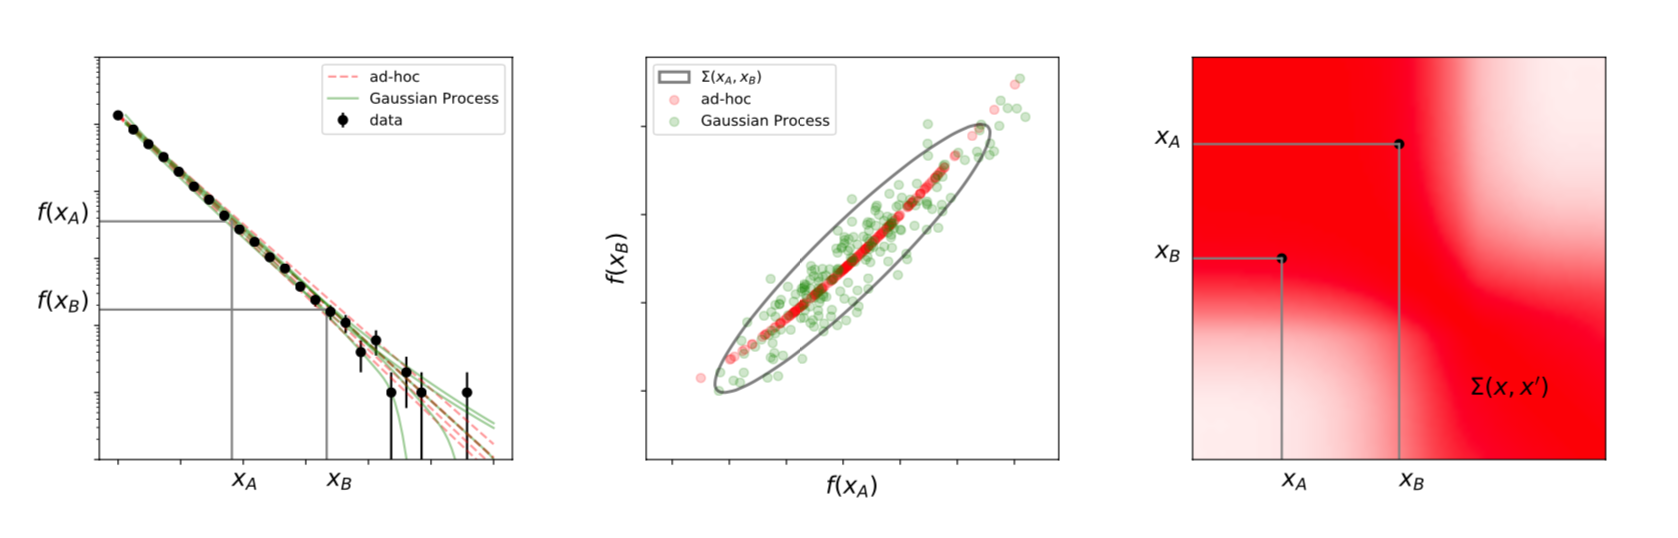
\includegraphics[width=0.7\textwidth]{figures/chapter_analysismethod/GP}
            \caption{
                These figure shows that the Gaussian process fit is able to provide more flexibility than the standard ad hoc fit~\cite{frate2017modeling}.
            }
            \label{fig:GaussianProcess}
        \end{center}
    \end{figure}
    \FloatBarrier


\subsubsection{Gaussian Process: Regression}

    The Gaussian process background prediction method is a Bayesian method, where the prior distributions can be "updated" by binning information from the MC/data histograms and a new prediction can be formed from the posterior. As the prior distribution in each bin is all approximated to be Gaussian distributions, it can be shown that the mean and covariance can be given by the following formulae:

    \begin{itemize}

        \item \textbf{The Mean Function}

    \begin{equation}
        \mu(x_{*}|y)  = \mu(x_{*})+ K(x_{*}, x)[K(x, x)+ \sigma^{2}(x)I]^{-1}(y-\mu(x))
    \end{equation}
    Here, $\mu$ is the mean function prediction of of point $x_{*}$, given known data point x and y, K is the kernel, and $\sigma$ is the white noise term.

    \item \textbf{The Covariance Function}
    \begin{equation}
        \sum(x_{*}, x_{*}') = K(x_{*}, x) - ((K(x_{*}, x')+\sigma^{2}I)^{-1)}[K(x, x')]
    \end{equation}  
    Here, the covariance is defined for $x_{*}$ and $x_{*}$, the data point where the predictions were made, x and x' where the input data points are given. K is the kernel of the Gaussian Process prediction.

    \end{itemize}

    Here, x and y are input data to constrict the distribution, $x_{*}$ is the points where the posterior GP are evaluated from, x' is the same points as x in a 2d matrix.

    Signal and Background prediction 
    \begin{equation}
        \mu_{bkg}(x_{*}|y) = \mu_{\textrm{bkg kernel}}(x_{*}|y)+K_{\textrm{bkg kernel}}(x_{*}, x) \cdot K_{\textrm{sig+bkg kernel}}(x,x') \cdot( y(x)-\mu_{\textrm{bkg kernel}}(x_{*}|y) )
    \end{equation}


    \begin{equation}
        \mu_{sig}(x_{*}|y) = K_{\textrm{sig kernel}}(x_{*}, x)\cdot K_{\textrm{sig+bkg kernel}}(x,x') \cdot ( y(x)-\mu_{\textrm{bkg kernel}}(x_{*}|y) )
    \end{equation}


\subsubsection{Gaussian Process: Covariance function}
\label{sec:kernel}
The covariance function/kernel describes how the joint distribution is related to each other in the Gaussian process. 
It's possible to embed different information regarding the physics of the spectrum into the kernel. 
In the dimuon analysis, it's found that the simple radial basis function and a white noise kernel are sufficient to describe the background spectrum, the signal is described by another radial basis function kernel of a particular mean value.
The kernels are given as the following: 

    \begin{itemize}
        \item \textbf{Background Kernel}

            The background kernel is the addition of the Radial Basis kernel function plus the white noise kernel.
            \begin{equation}
                K_{bkg}(x, x') = A_{1} * exp(-\frac{||x-x'||}{2\sigma^{2}}) *+ K_{noise}
            \end{equation}
            Here, $A_{1}$ is the amplitude hyperparameter that describes the size of the kernel, $\sigma_{1}$ is the lengthscale parameter.
            The noise kernel is a constant diagonal kernel:
            

			\begin{equation}
            K_{noise}(x_{i}, x_{j}) =
			\begin{cases} \text{noise level} & \text{if $x_{i}==x_{j}$,} \\
			\\
            0 & \text{otherwise.}
			\end{cases}
			\end{equation}

        \item \textbf{Signal Kernel}

            The signal kernel is a square centered exponetial kernel
            \begin{equation}
            K(x_{i}, x_{j})=A_{2}\cdot exp(-(x-m)^{2}/(2\cdot\sigma_{2}^{2}))\cdot exp(-((x'-m)^{2}/(2\cdot\sigma_{2}^{2}))) + K_{noise}
            \end{equation}

    \end{itemize}
            Here, $A_{2}$ is the amplitude of the signal kernel, m is the value where the kernel peaked on, and $\sigma_{2}$ is the lengthscale of the signal kernel. 
    \subsubsection{Gaussian Process: Hyperparameter Optimization}
    The kernels hyperparameter are optimized by minimizing the negative log marginal likelihood of the Gaussian Process:

    \begin{equation}
        -logL = -\frac{1}{2} log |\sum| - (y-\mu(x) ) - \frac{n}{2}log(2\pi)
    \label{eq:loglikelihood}
    \end{equation}
    
    In the dimuon analysis, the minimization is done through initialization of hyperparameter from first a grid search and then scalar conjugate gradient search, the different results are compared with each other for the optimized hyperparameter set.

    In this Gaussian process testing procedure, the hyperparameters are first found on a test fit on the MC/data, a minimum bound on the lengthscale hyperparameter is first found through a fit on different variations of the MC generated and the signal injected test.

\subsubsection{Gaussian Process: Background Fitting}
In Gaussian Process, the background fitting's validity is tested by different methods. First, the signal injection test 

\subsection{Signal Injection Test}
    \label{sec:signalInjection}
    An increasing number of parameters in a fit or number of windows in SWiFT provide more flexibility in modelling the background accurately. However, the increased flexibility in background modelling often comes with the price of decreased signal sensitivity: the flexible background fits the signal away as part of the background. The signal injection test is a test that quantify the amount of signal sensitivity in the chosen background modelling. On ATLAS, it is required that the background modelling provide sensitivity to signals of at least 3 $\sigma$ of the background error, defined by the width of the Gaussian envelop on the fits done on the pseudo-experiments. In additional to quantifying signal sensitivity, in Gaussian process and the SWiFT background estimation, the signal injection test is used to constrain the lower bound of the lengthscale and SWiFT window, finding the hyperparameter or parameter that would return a background that provides the signal sensitivity. 

    The procedure in this thesis uses bumphunting~\cite{choudalakis2011hypothesis} with each background fit.
   For each chosen maximum lengthscale/SWiFT window, and different signal widths, the below is performed:

   1. First a background fit is performed on the bacground MC, the bump-hunting is performed as described in the above section. If the overall bumphunter p-value is below the critical value for window exclusion, the next step is performed. Otherwise, another background fit is looked for.

   2. A small signal is injected in the background MC, a fit is reperformed, and the bumphunter window and overall p-value is calculated again. 

   3. An increasing signal size is injected into the spectrum, step2 is repeated, until a signal of size large enough to lead to a small enough p-value where window exclusion in the bumphunting procedure gets triggered. The signal size injected just before the window exclusion is the largest signal the search is not sensitive to. The minimal signal size injected that triggers the window exclusion is the smallest signal size that the search is sensitive to. 

\begin{figure}[!htb]
    \begin{center}
        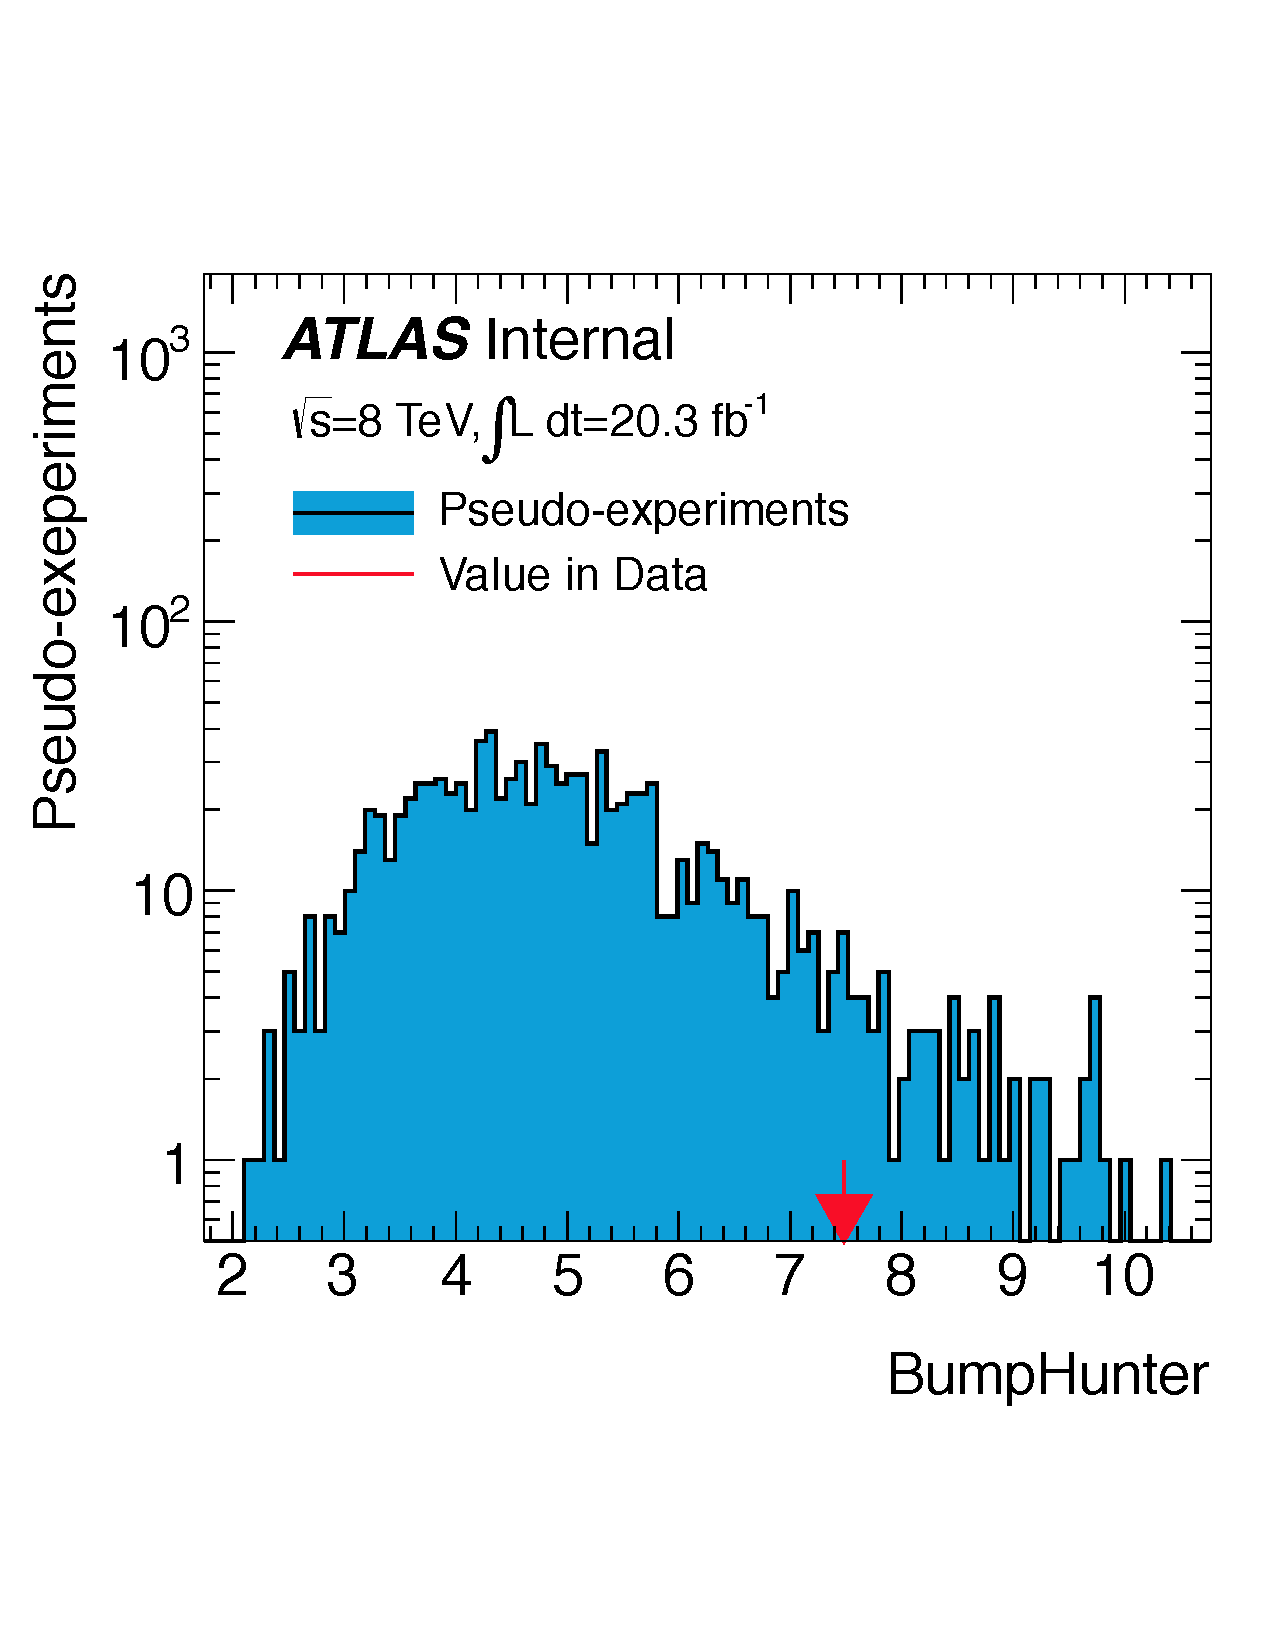
\includegraphics[width=0.75\textwidth]{figures/chapter_analysismethod/bumphunter}
        \caption{
            This diagram shows the bumphunter test statistics distribution, where the red arrow shows the observed value. 
        }
        \label{fig:teststats}
    \end{center}
\end{figure}
\FloatBarrier
   
   The background fit, or parametrically, the SWiFT window size/Gaussian process lengthscale, is said to have passed the test if the largest signal the search is not sensitive to is within 3 $\sigma$ of the background error bands. 

   The smallest lengthscale value/SWiFT window size where the largest signal the search is not sensitive to stays in the error bands is the minimal SWiFT window/Gaussian Process fit value that can be used during unblinding. 

\begin{figure}[!htb]
    \begin{center}
        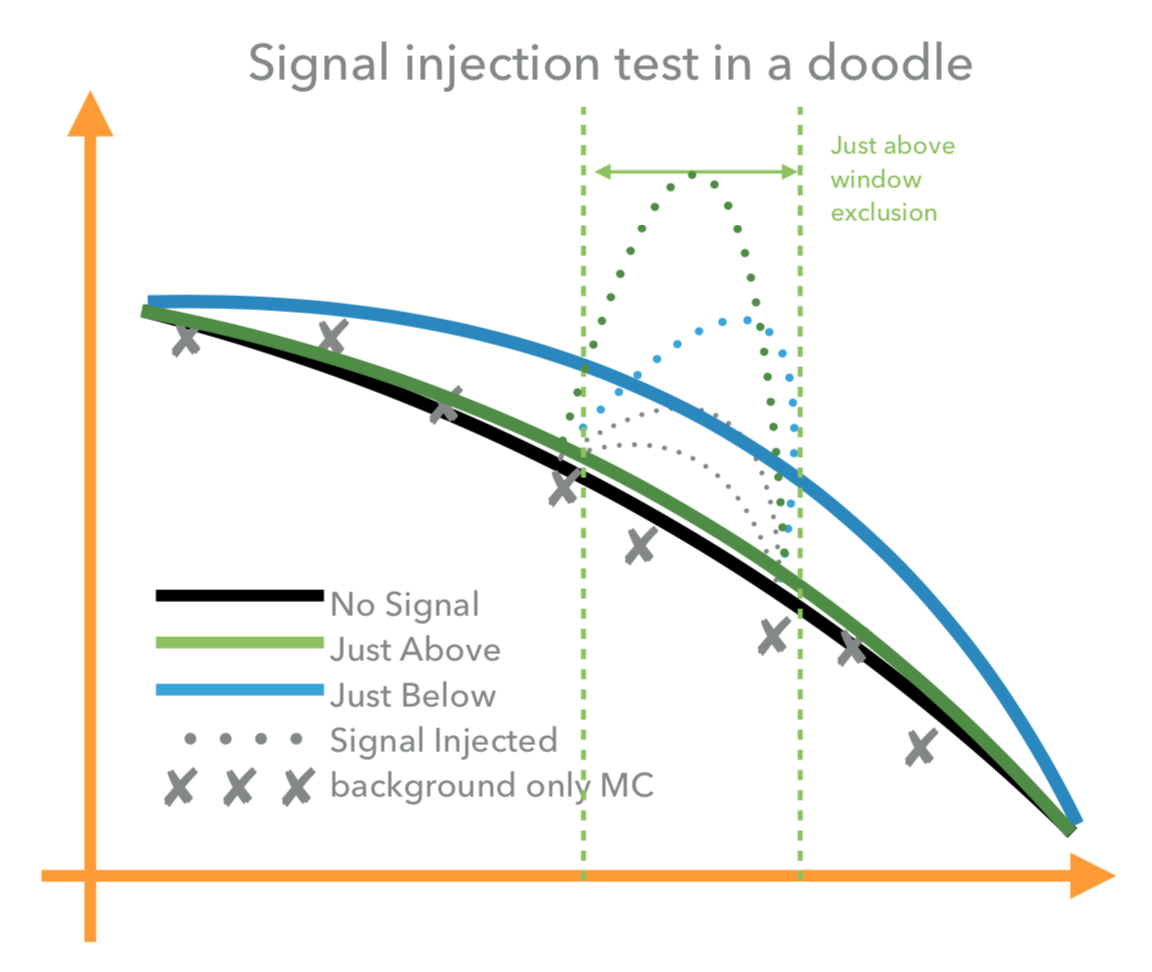
\includegraphics[width=0.7\textwidth]{figures/chapter_analysismethod/SignalInjectionTest}
        \caption{
            This figure shows a doodle on the procedure of the signal injection test.
        }
        \label{signalinjection}
    \end{center}
\end{figure}
\FloatBarrier

    \subsection{Spurious Signal Test} 
    \label{spurious}
    To measure the amount of possible false signal that is captured by the background modelling method, the spurious signal test is done. The spurious signal test models the amount of signal that the background plus signal fit when no signal is present.  It's a statistically quantify the stability of the background estimation. It is also sometimes used as a measure of the background fit error.

    A thousand independent background plus signal fit is performed on pseudo-experiments generated from the background MC. The spurious signal is defined as the following:
    
    \begin{equation}
        S_{spur} = S_{fit} - S_{template}
    \end{equation}

    Here $S_{fit}$ comes from the signal fit component of the background + signal fit, $S_{template}$ changes with the kind of analysis being performed. It is set to be 0 for a search. 
    The median of the 1000 pseudo experiment fit is taken to be the spurious signal value. 
    In the figure below, a sample spurious signal fit is shown~\ref{spurioussignal}.
    In general, the spurious signal has to stay within 50\% of the background error bands, defined as the error bands generated from the fitting of 10000 background MC pseudo experiment from the Poisson distribution with the background fit only.
    If the background fit stays within the 50\% requirement, it passes the spurious signal test, otherwise, it doesn't. 

\begin{figure}[!htb]
    \begin{center}
        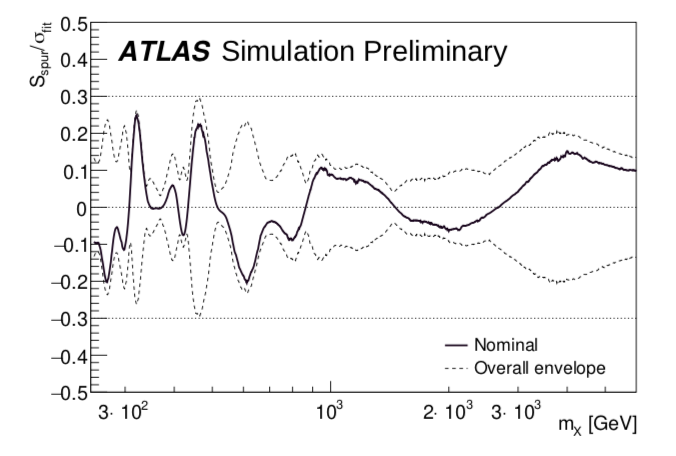
\includegraphics[width=0.75\textwidth]{figures/chapter_analysismethod/Spurious}
        \caption{
            This figure shows the example results of a spurious signal test. Here, the error $\sigma$ is defined as $\sigma_{tot} = \sqrt{\sigma^{2}_{fit}+ S_{spur}^{2}}$ ~\cite{ATL-PHYS-PUB-2020-028}.
        }
        \label{spurioussignal}
    \end{center}
\end{figure}
\FloatBarrier

    \subsubsection{Gaussian Process: Limit Setting}

    The Gaussian process is shown to be able to be incorporated within the Asimov method of frequentist limit setting in section~\ref{sec:freq}. The Asimov limit is a frequentist limit calculation method that saves on computing resources. The limits are generated from a representative asimov dataset instead of a the full dataset of all values.
    In the graph~\ref{fig:chi2}, the Likelihood ratio in Gaussian process is a proxy for the profile likelihood ratio used in the Asimov limit. It can be seen that it approximately follows the $\chi^{2}$ distribution, satisfying a requirement that follows from the Wald approximation that allows for the Asimov approximation of limits.
    More details on the derivation and the use of asimov limit can be found in the following section~\ref{sec:asimov}.

    \begin{figure}[!htb]
        \begin{center}
            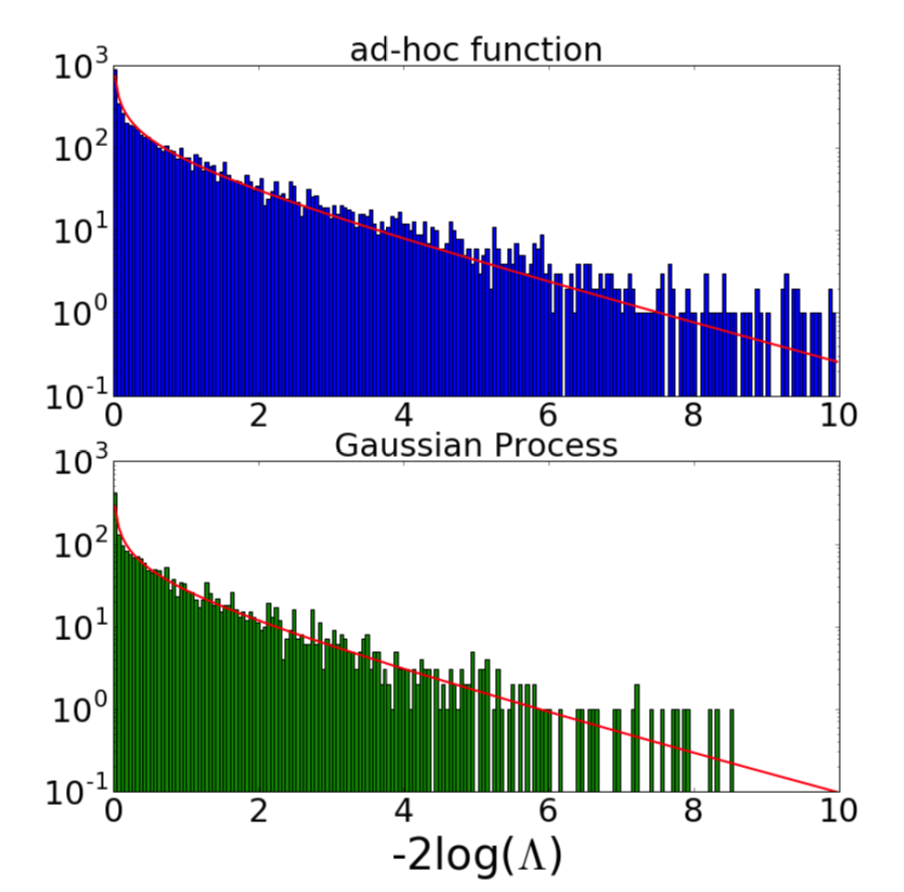
\includegraphics[width=0.75\textwidth]{figures/chapter_analysismethod/chi2}
                \caption{
                This figure shows the negative log of the $\Lambda$ which is an approximation of the measure of the profiled likelihood ratio defined in~\ref{eq:profilelikelihood}. The top part is the distribution for background only pseudoexperiments, whereas the bottom is the background + signal distribution. They show a reasonable agreement to the $\chi^{2}$ fit, a required condition for the Asimov approximation for a frequentist limit setting in
            section~\cite{frate2017modelling}. }
            \label{fig:chi2}
        \end{center}
    \end{figure}
    \FloatBarrier

\section{Statistics Testing}
\label{section:stats}
Statistical testing is the quantification of whether an excess is seen or what experimental bound can be drawn from the final analysis. 

The statistics testing on a hypothesis can be presented as a test on the significance Z: 

\begin{equation}
 Z= \Phi^{-1}(1-p) 
 \label{eq:significance}
\end{equation}

Here, p is numeric probability representation of the agreement between the data and the model given a hypothesis. $\Phi$ is its conversion of the p value in to quantile of on a cummulative Gaussian distribution. This formula is central to all statistical hypothesis testing done. From here on, Z will be referred the significance and p will be referred to as the p-value with regards to the experimental hypothesis. 

There are two distinct statistics test that are done in a typical resonance search analysis. Each test is done on a threshold value of Z. The two tests will be referred to as "the search" and "the limit setting" from here on. The details on the two statistical test are descibed in the following section.

%Before the Here, the null hypothesis is the hypothesis that include only known processes from the Standard Model hypothesis with no excess; the alternative hypotheis is the hypothesis that include both background and signal of a certain signal strength.

%\begin{itemize}
%    \item \textbf{1.  The Search}
%()corresponds to $p = 2.87 \cdot 10^{-7}$.


%the Bayesian tool is used for the dijetISR analyses, whereas the frequentist method is used for the dimuon analysis. 
%\end{itemize}

\subsection{The Search}


\textit{Rejection of the null hypothesis}
The statistical search test for excesses is called the search. This test is done on the null hypothesis, where it's defined to be the Standard Model prediction. If the given data return a value, as calculated from ~\ref{eq:significance} Z \> 5, the null hypothsis is rejected, something beyond the Standard Model is observed in the data to a statistically significant degree. The rejection test is also called the discovery test. For example, in the Higgs boson analysis of 2012, a significance of Z\> 5 was observed in the search. However, note that the rejection of the null hypothesis is a necessary condition but not a sufficient condition for discovery.

The search is done by in a frequentist manner through the Bumphunter method~\cite{choudalakis2011hypothesis} for both the dimuon and dijetISR analysis. This section will first go over the statistics principle behind resonance finding, then on the defined bumphunter test statistics, lastly on the bumphunting procedure. 





\subsubsection{The Search: The Statistics Principles}

The statistics of the Standard Model prediction given the observed measurenment in each bin can be described by a probability distribution. As each count is considered an independent event in a fixed data taking period and physical variable value. It's probability is given by the Poissonian probability distribution:

\begin{equation}
 P(x|\lambda) = \frac{\lambda^{k}e^{-\lambda}}{k!} 
 \label{eq:Poissonian}
\end{equation}

Here, Lambda is the expected value of the measured quantity x, k is the number of occurences, e is the Euler's number  

    The test is done in a frequentist manner, it compares the observation outcome x with a fixed critical value $\alpha$ of a probability distribution generated from pseudo-experiment from a Poisson distribution. The value used to reject or accept the null hypothesis is a probability quantity called the p-value. Statistically, it is known to be a false-discovery probability. 
    If the observation compared with the distribution outcome is smaller than the critical p-value, the null hypothesis is rejected. The rejection criteria can be shown in the following mathematical form:

\begin{equation}
    P(x \ni w|H_0)<= \alpha 
    \label{eq:test}
\end{equation}


Here, $H_0$ is the prediction from the null hypothesis, and alpha is the critical value below which the null hypothesis will be rejected. The value is usually taken to be 0.01 for the bumphunter experiment. 

\subsubsection{The Search: Test Statistics}
\label{teststatistics}

The test statistics is a function of the observable x, the p-value in~\ref{eq:test} can be rewritten as such:
    
\begin{equation}
    p = P(T>=t_{0}| H_{0})
\label{eq:p-valuetestStats}
\end{equation}

Here, $H_0$ is the null hypothesis prediction, $t_0$ is the test statistics of the null hypothesis, and T is the observed test statistics.


If the test is concern with how well the data fits the model alone, the test statistics can be chosen to be either the $\chi^{2}$ test or the log-likelihood of the Poissonian distribution. These quantities can be directly derived from the Poissonian probability in ~\ref{eq:Poissonian}. They provide information about the overall fit. As the search specifically looks to quantify the deviation between the data and the prediction as a bump, they are not the optimal choice for the test. 
The bumphunter test statistics, which is defined in a window of neighboring bins, is used instead to best describe the kind of deviation expected in excesses seen in neighboring bins. The derivation is given below: 

In a window defined from bin number m to n, the observed data and prediction can be given as the following: 
    \begin{equation}
         d= \sum_{i=m}^{n} d_i 
    \end{equation}

    
    \begin{equation}
         b= \sum_{i=m}^{n} b_i
    \end{equation}

    Here d is the total number of events in the window observed, where $d_i$ is the count in each of the bin from m to n. 
    Here b is the total number of events in the window predicted, where $b_i$ is the event count in each of the bin from m to n.
    
    Assuming the observed counts in each bin follows a Poisonian distribution, the test statistics is as the following:

	\begin{equation}
    t=
	\begin{cases} \sum_{n=0}^{d} %\frac{b^{n}}{n!} e^{-b}%&\textrm{for $d < b$}
    %\sum_{n=d}^{\infinity} \frac{b^n}{n!}e^{-b}%&\textrm{for $b \leq d$}.
    \end{cases}
    \end{equation}

    The above expression can be represented by the Gamma function: 

	\begin{equation}
    t=
	\begin{cases} 1-\gamma(d+1, b)%& \textrm{for $d < b$}
    \\
    \gamma(d,b)%  & \textrm{for $b \leq d$}.
    \end{cases}
    \end{equation}
    


    From this test statistics, equation~\ref{eq:p-valuetestStats} can be used to evaluate the p-value of the observed value. T is calculated directly given the observed x in the window, and $T_{0}$ is given by generating poissonian fluctuation from the fit background model. T is compared against the psuedoexperiment value of the test statistics, and p is found that way for each window. 

    In each Bumphunter scan, the p-value of the bumphunter test statistics is evaluated for windows sized from two-bin wide to half the spectrum, this gives information on the localized excesses seen in each window.

    The overall bumphunter test statistics is defined by the to be the log of the smallest p value calculated from the most deviant window. The test statstiscs can be represented as the following:

    \begin{equation}
        t_{0} = - ln (t_{min}) 
    \end{equation}

    Significance Z and the p-value can be calculated from this test statistics in equation~\ref{eq:p-valuetestStats} and thereby provide an overall bumphunting deviation from the Standard Model. If the p-value is lower than 0.01, the null hypothesis is rejected. An excess would be claimed. 

    In addition to the bumphunter test statistics, there is the tailhunter, KS, Jeffreys and no sidebands bumphunter that can also be chosen for different signal searched for in other physics analyses. More information can be found in the Bumphunter paper\cite{choudalakis2011hypothesis}.

    \subsubsection{The Search: The Bumphunting Procedure}
    % Look up the bumphunter fit. 
    The bumphunting procedure is a set of procedure defined to look for excesses from the bumphunter statistics defined above. The following is cited from this source\cite{Pachal:206032}.

    1.  First a background model fit is performed, from the method illustrated from the fit method session~\ref{sec:backgroundest}. The $\chi^{2}$ of the fit has to have a p-value $>$ 0.01. Otherwise, the fit will be revised or move to an alternative method.

    2.  If the background fit passes the $\chi^{2}$ test, the bumphunting test statistics can be evaluated. In all the windows across the spectrum, Bumphunter test statistics and their p-values are calculated. If the overall bumphunter test statistics has a p-value above 0.01, stop, no excesses is found. Alternatively, if any one of the window goes below p< 0.01, the window most discrepant window (the window with the lowest p-value) is removed, and the fit is reperformed.

    3. If an overall bumphunter statistics p-value is found to be less than 0.01, the most discrepant window is removed. A background fit is reperformed without the window. The bumphunter statistics and the pvalue is recalculated for the window sets, if all found bumphunter p-value is above 0.01, stop. A bump is likely "discovered" in the removed window. Otherwise, if the p-value is below 0.01, see if the most discrepant window in the new scan is adjacent to the removed window, if yes, add the adjacent two bin (left and right) to the fit. This step is repeated. until either the p-value of the fit outside the window goes above 0.01, or no additional window could be added to the exclusion. If not, the fit needs to be re-evaluated.

    Summarizing from the above, three end results are possible in the search test:

    1. If no window is excluded and the fit has a bumphunter p-value statistics above 0.01, the null hypothesis is accepted. No beyond the standard model excess is found. 

    2. If there is one excluded window and a background fit with a bumphunter statistics p-value of >0.01, the null hypothesis is rejected, an excess may be seen. 

    3. In all other sceanrios, more tests needs to be done. The background model fit could be problematic and need further testing.  

\section{The Limit Setting}

\textit{Finding signal strength value where the alternative hypothesis is rejected to a 95\% confidence level}

If no excesses is found in the previous step in the Search, limit setting is performed. Limit setting a statement on the signal strength that the analysis has confidently rejected. Statistically, the upper limit setting is the finding of the signal strength where the alternative hypothesis is rejected at 95\% confidence level. The signal strength can also be represented as a cross section or cross section in fidicial volume for reinterpretation for different models. 
The limit setting results consist of a 95\% confidence upper limit line and an expected limit of median significance along with a 3 $\sigma$ and 5 $\sigma$ significance band. It is possible to compare the observed 95\% upper limit against the expected limit. The comparison between the bands and the upper limit line can be seen as a discovery test, as if no beyond the Standard Model excess is seen, the upper limit line would stay between the 5 $\sigma$s error band in the expected limit. 

In ATLAS, the limit setting can be done in two different way, the Bayesian statistical way and the frequentist way. While the interpretation and implication of the results made with the different methods are different, the results produced are interchangeable and can be compared across different analyses. 
The Bayesian method is used for the dijetISR analysis and the frequentist method is used for the dimuon analysis, a description of both of them are given as below.
%The 95\% confidence level corresponds to a critical p-value of 0.05 or a Z value of 1.64.

%The limit is a hypothesis testing procedure that test both the compares the null hypothesis of absence of signal ($H_{0}$) to the hypothesis where there is a signal($H_{1}$). 
%The limit is a projection of the $H_0$ and $H_1$ hypothesis in either the cross-section or the signal strength axis. This provide another way to discuss signal discovery, and information on an 95\% confidence limit in the If $H_1$ shows agreement with $H_{0}$ when fluctuation is taken into account, the 
%Even in the absence of a signal, a statement can be made about the signal strength value that is ruled out by the signal+background. 
%
%The limit setting procedure can be done in both the frequentist and Bayesian way on ATLAS, and in the analyses presented, the dimuon analysis is done in the frequentist way, whereas the dijet analysis is done in the Bayesian way. 

%\subsection{Bayesian limits}


\subsection{Frequentist Limits}
\label{sec:freq}
In the frequentist sense, all events are considered indepedent events in possible worlds. The limit is a statement on where the observed data lies given all the other possible outcome given a hypothesis. 
The following subsection describes the test statistics used for the limit setting in ~\ref{sec:freqTestStats}. It gives a formulation of the traditional frequentist calculation. In~\ref{sec:asymp} and ~\ref{sec:asimov} the Asimov approximation method used to approximate the frequentist limit from a representative dataset is described, which is the ATLAS standard on saving computing resources. The formulae for the limit calculation using this method is given in the end
in~\ref{sec:asimov}.

\subsubsection{The Frequentist Limits: The Test Statistic}
\label{sec:freqTestStats}

The probability distribution of the observable x histogram can be given as a Poissonian distribution. The predicted model on x can be described by both the signal strength parameter along with other nuissance parameters. Extracting only the parameter dependent part of the Poissonian probability distribution function, a likelihood function is obtained:

\begin{equation}
    L(\mu, \theta) =  \prod_{i=0}^{N} \frac{(\mu s_{j} + b_{j})^{n_j}}{n_{j}!}e^{-\mu s_j + b_j} \prod_{k=1}^{M}\frac{u_{k}}
{m_{k}!} e^{-u_{k}}
\label{eq:likelihood}
\end{equation}

Here, $L$ is the likelihood product from the target distribution multiplied by the constraint distribution, $\mu$ is the signal strength, $s_j$ is the number of signal events in each bin, $b_j$ is the number of background event in each bin, $n_j$ is the number of observed event in each bin in the targetted signal distribution; N is the total number of bins in the targetted observed distribution. The likelihood is also affected by by terms in other distributions, these
are not the target distribution and can be accounted for as the nuissance parameters, which
includes:
here $u_k^{m_k}$ is the predicted value by the model, and $m_{k}$ is the observed value. 

When the likelihood function is maxmimized, gives the most optimal value of all the parameters. However, since in limit setting, the only parameter we are interested in learning about is the signal strength, the influence from the unknown truth value of the nuissance parameters can be taken into account or eliminated. A profiled likelihood function is constructed to achieve this. This quantity, when maximized, gives the overall most likely signal strength prediction while taking into account fluctuations in the other nuissance parameters. 

\begin{equation}
\lambda(\mu) = \frac{L(\mu, \hat{\hat{\theta}})}{L(\hat{\mu}, \hat{\theta})}
\label{eq:profilelikelihood}
\end{equation}

Here, the denominator is the maximized unconditional likelihood function, where $\hat{\mu}$ and $\hat{\theta}$ is the parameter values that would maximize the unconditional likelihood function; the nominator is the conditional likelihood function, that would be maximized under the maximum-likelihood estimator of $\theta$ and $\mu$. 

%To aid the optimization process and also to reflect the nature of the excess search experiment that neglects negative signal event value, the test statistics defined as the following, the negative log taken on the likelihood ratio aid the optimization computing procedure.
To aid the optimization process, it's usually the negative log of the profiled likelihood that is used for the limits calculation:

\begin{equation}
    q_{\mu} = -2 ln \frac{L(\mu, \hat{\hat{\theta}})}{L(\hat{\mu}, \hat{\theta})}
\label{teststats}
\end{equation}


\subsubsection{The Frequentist Limits: The Limits Formulae}
\label{sec:limits}

From this test statistics, the p-value calculated from the different assumed signal strength and observed data can be found, the signal strength where the data can reject up to 95\% is called the observed limit, and the signal strength of median significance along with the fluctuation is called the expected limit. 

\begin{itemize}


\item \textbf{The Observed 95\% Upper Limit}
\begin{equation}
\mu_{up/lo} = \hat{\mu} +- \sigma\Phi^{-1}(1-\alpha/2)
\end{equation}

\item \textbf{The Expected Median Limit}
\begin{equation}
    med[\mu_{up}|\mu'] = \mu' + \sigma\Phi^{-1}(1-\alpha) 
\end{equation}

\item \textbf{The Error Band}
\begin{equation}
    band_{N\sigma} = \mu' + \sigma(\Phi(1-\alpha)+-N)
\end{equation}

\end{itemize}


Here, $\mu$ is the signal strength being considered, $\alpha$ is the significance associated with 95$\%$ confidence and the median significance repectively, $\Phi$ is the cummulative Gaussian distribution where the observed p-value lies.

Note that the calculation of the denominator in~\ref{eq:likelihood} is CPU intensive, and can be approximated with a representative distribution as described in the following section.


\subsubsection{The Frequentist Limits: The Asymptotic distribution}
\label{sec:asymp}


Using the Wald theorem the test statistics can be approximated: 

\begin{equation}
-2ln(\lambda(\mu))= \frac{(\mu- \hat{\mu})^{2}}{\sigma^{2}} +O(1/\sqrt{N})
\label{eq:wald}
\end{equation}

Here, $\mu$ is the observed value, whereas the $\hat{\mu}$ is the expected strength that would maximize the likelihood, $\sigma$ is the expected spread in the distribution. 

If the terms in O are neglected, it follows that the test statistics will then asymtotically follow a non-central chi-square distribution: 

\begin{equation}
    f(q_{\mu}) = \frac{1}{2\sqrt{q_{\mu}}} \frac{1}{\sqrt{2\pi}} [exp(-\frac{1}{2}(\sqrt{q_{\mu}}+ \sqrt{\Lambda})+ exp(-\frac{1}{2}(\sqrt{q_{\mu}-\sqrt{\Lambda}})^{2})]
\end{equation}
Here, $\Lambda$ is the non-centrality term, it can be shown that it can be estimated to be:

\begin{equation}
    \Lambda=2ln(\lambda_{A}(\mu))
    \label{eq:Lambda}
\end{equation}

A detailed proof can be seen in the following reference \cite{2011}. 

%\[ \lambda_{A}(\mu) = \frac{L_{A}(\mu, \hat{\hat{\theta}})}{L_{A}(\hat{\mu}, \hat{\theta})} \]


%Following certain estimation, the non-centrality term, \Lambda, can be given by the following:


%Following from this, it can be shown mathmatically the median significance, the error bands, as well as the upper limit exclusion can be given as the following: 


%The upper limit is given by: 
%\[ \

%The median significance of the expected limit is given by
%\[ \Lambda = \frac{(\mu- \hat{\mu})^{2}}{\sigma^2}=-2ln{lambda} \], where mu is the expected value, this is known as the asimov dataset. 


%\begin{figure}[!htb]
%    \begin{center}
%        \includegraphics[width=0.75\textwidth]{figures/chapter_analysismethod/asimovApproximation}
%        \caption{
%			Generation showing convergence of the Asimov dataset and the median significance dataset from full generation. .
%        }
%        \label{fig:Model_figure}
%    \end{center}
%\end{figure}
%
%
%\[ Z^{2}_{median} = -2ln{\lambda_{median}} \]
%
%As can be shown from the MC generation plot here, the median conversed 
%
%Using the above approximation, one distribution can be used instead of a large amout of ensemble data, the above is known as the Asimov dataset. 


%There are some special cases where the 

%From the Wilk's theorem, the upper limit on the signal strength $\mu_{95}$ can be given as the following:


\subsubsection{The Frequentist Limit: The Asimov dataset}
\label{sec:asimov}

The finding of $\hat{\hat{\mu}}$ in the denominator in the test statistics in equation ~\ref{teststats} is CPU intensive, the dataset is large with many dimensions. The asimov dataset reduces the calcuation here by showing that $\hat{\hat{\mu}}$ can be approximated by $\mu'$, the expected value of the strength parameter. From this, CPU intensive calcuation of the p-value, significance and thus the upper limit and its fluctuation can be reduced to simple formulae that only look at the representative Asimov dataset. 
A proof is given as the following section, and the formulae used for upper limit and expected limit calcuation in this thesis is included in the end. 

From the definition, true values of parameters will result in a maximum likelihood and therefore the derivative of the ${L}$ will be equal to 0. 

\begin{equation}
%\frac{\partial{L}}{\partial{\theta_{j}}} %\sum_{i=0}^{N}(\frac{n_{i}}{\nv_{i}}-1) \frac{\partial{\nv_{i}}}{\partial{\theta_{j}}}+ \sum_{i=0}^{N}(\frac{m_{i}}{u_{i}}-1) \frac{\partial{u_{i}}}{\partial{\theta_{j}}} =  0 
\end{equation}

Here, n is the number of count in the bin in the signal region variable x, and N is the total number of bins, and m is the number of counts in the bin in the control region may help further constrain the background, M is the maximum number of bins. 

The maximal likelihood value for $n_{i,A}$ and $m_{i,A}$ is associated with their expectation value. 

\begin{equation}
    %n_{i,A} = E[n_{i}] = \nv_{i} = \mu s_{i}(\theta) + b_{i}(\theta)
\end{equation}

\begin{equation}
    %m_{i,A} = E[m,i] = u_{i}(\theta)
\end{equation}


These optimal parameters $\theta$ can be estimated through large size Monte Carlo generation. And it's called the asimov dataset.
The only missing part from the above estimation is $\sigma$ and it can be approximated as the following: 
Since, 

\begin{equation}
    \lambda_{A}(\mu) = \frac{L_{A}(\mu, \hat{\hat{\theta}})}{L_{A}(\hat{\mu}, \hat{\theta})}
= \frac{L_{A}{\mu, \hat{\hat{\theta}}}}{L_{A}(\mu', \theta)}
\end{equation}


From equation~\ref{eq:wald} and ~\ref{eq:Lambda}:
\begin{equation}
2ln(\lambda_{A}(\mu)) \approx \frac{(\mu-\mu')^{2}}{\sigma^{2}}=\Lambda
\end{equation}

$\sigma_{A}$ can therefore be approximated as the following:

\begin{equation}
    \sigma_{A}^{2} = \frac{(\mu-\mu')^{2}}{q_{\mu,A}}
\end{equation}

When there is no signal, $\mu'$ is taken to be zero. 


Once that's found, the likelihood profile of the search can be estimated through the Asimov likelihood as such:

Following from the above, the test statistics, the upper limits, the discovery median significance can all be found through substituting $\hat{\mu}$ as $\mu'$ by the asimov method. As these result derives directly from the above, only the results are quoted here. 

\begin{itemize}
    \item \textbf{The Test Statistics Distribution}

\begin{equation}
    F(t_{\mu}| \mu) = 2\Phi(\sqrt{t_{\mu}})-1
\label{eq:teststatistics}
\end{equation}

Here F is the distribution of the statistics, $t_\mu$ is the test statistics at the given $\mu$ value of the distribution. 

\item \textbf{The P-value of a Hypothesized $\mu$ for an Observed Value $t_\mu$}

\begin{equation}
p_{\mu} = 1-F(t_{\mu}| \mu)=2(1-\Phi(\sqrt(t_{\mu})))
\end{equation}


\item \textbf{The Significance that Corresponds to the Above p-value}

\begin{equation}
Z_{\mu} = \Phi^{-1}(1-p_{\mu})  = \Phi^{-1}(2\Phi(\sqrt{t_{\mu}})-1)
\end{equation}

\end{itemize}

From this calculation, the limit calculation in the above~\ref{freq:limits} can be utilized for an limit calculation. 

%\subsection{The Search (discovery test)}
%A hypothesis is said to be rejected if its p-value is below a certain threshold z value of alpha. This is the basis of the discovery test.
%Using the test statsitics:
%
%
%
%\begin{equation}
%\[ Z_{0}= \Phi(1-p_{0})= \sqrt(q_{0}) \]
%\end{equation}



%In the experiment, statistical fluctuation need to be taken into account, it can either be taken as that the data has room to fluctuate, or that the expected value from the model can fluctuate and change. Either way, the sigificance will fluctuate even if $\mu'$ is assumed to be true and hold fixed. In the analysis, it's taken that data will be fluctuating. 
%
%In the case where there is assumed that there is no background. Using the fluctuation, the significance can be calculated as the following: 
%
%\begin{equation}
%Z_{0}= 
%\begin{cases}
%    1& \text{\mu* \sigma    \hat{\mu}\gt 0}
%    2& \text{0    \hat{\mu}<0}
%\end{cases}
%\end{equation}


%For the expected limit test, the significance can be written as:
%\begin{equation}
%    \[ Z_{0}(\mu'+N\sigma) = med[Z|\mu'] +N \] 
%\end{equation}
%

%\begin{equation}
%    \[ max[Z_{0}(\mu'+N\sigma) = med[Z|\mu'] -N, 0] \] 
%\end{equation}

From the above formulation, it can be shown that the limit can be caculated analytically following the generation of an Asimov dataset, thus saving a lot of computaion power from the full limit generation. 

\subsubsection{The Frequentist Limits: The Gaussian Process Adaptation}

In Gaussian Process, a few adaptation is made to the original Asimov frequentist approximation shown in the last section. First the test statistics is swap out:

\begin{equation}
    -ln(\Lambda), where \Lambda= 2ln(\frac{L_{\textrm{GP signal + bkg fit}}(\mu, \hat{\hat{\theta}})}{L_{\textrm{GP bkg fit}}(\hat{\mu}, \hat{\theta})})
\end{equation}

Here, $\ln(\Lambda)$ is the new test statisitics used for the limit setting L is the likelihood defined in Eq.~\ref{eq:loglikelihood}. The nominator is the likelihood with both the background and signal kernel, whereas the denominator is likelihood with just the background kernel. 

Using this newly defined test statistics, Eq.~\ref{eq:teststatistics} does not hold, and the test statistics may not always follow the $\chi^{2}$ distribution in Figure~\ref{fig:chi2}. The test statistics either has to be cross checked or reweighted. When this requirement is satisfied, Gaussian Process and its test statistics can use the approximation listed out in the above section for Asimov limit setting.


%\section{Systematics}
%\section{Future Extensions}


